\section{LITERATURE REVIEW}
\label{sec:literature_review}
\subsection{LiDAR}
\label{subsec:lidar}
The sensing system for automated vehicle navigation is made up of active and passive sensors, such as cameras, radar, and lidar~\cite{lidar}.
One such device LiDAR, is an advanced active sensor system that uses lasers to illuminate 
and detect its surroundings. These devices measure distances to various objects precisely 
by emitting lasers and receiving them back from reflective surfaces. 
In a typical LiDAR system, one or more laser beams are scanned across its field of view. 
The generation and control of these laser beams is dependent on a sophisticated beam control system.
Lasers are typically created using modulated laser diodes that emit light at near-infrared (NIR) wavelengths. 
The laser beams are then reflected back by objects in the environment, and the resulting signals are captured by photodetectors on the scanner. Fast electronics in the lidar system filter these returned signals and calculate the time difference between the emitted and received laser light. 
This time difference is the key to calculating the distance because it is proportional to it. 
This time difference enables the system to precisely estimate the distance between the laser and the object. 
Furthermore, advanced signal processing techniques can compensate for variations 
in reflected intensity caused by differences in surface materials or environmental conditions 
between the transmitter and receiver. 
LiDAR typically produces a point cloud of data that depicts the structure of the scanned environment 
and includes information on each point's location as well as the intensity of the reflected laser energy. 
This makes LiDAR extremely useful for environmental modelling and object recognition.
LiDAR ranging is capable of working in two modes: direct detection and coherent detection. 
Direct detection laser rangefinders are devices that use a pulsed laser 
to directly measure distance by measuring the laser's time of flight (ToF). 
The other type of device, known as a coherent detection laser rangefinder, 
uses a Frequency Modulated Continuous Wave (FMCW) laser 
to indirectly measure an object's distance and speed using the Doppler effect~\cite{lidarintro}. 

The LiDAR system used in this project is a typical kind of ToF LiDAR, whose working principal is shown in Figure~\ref{fig:lidar_example}.

\begin{figure}[H]
    \centering
    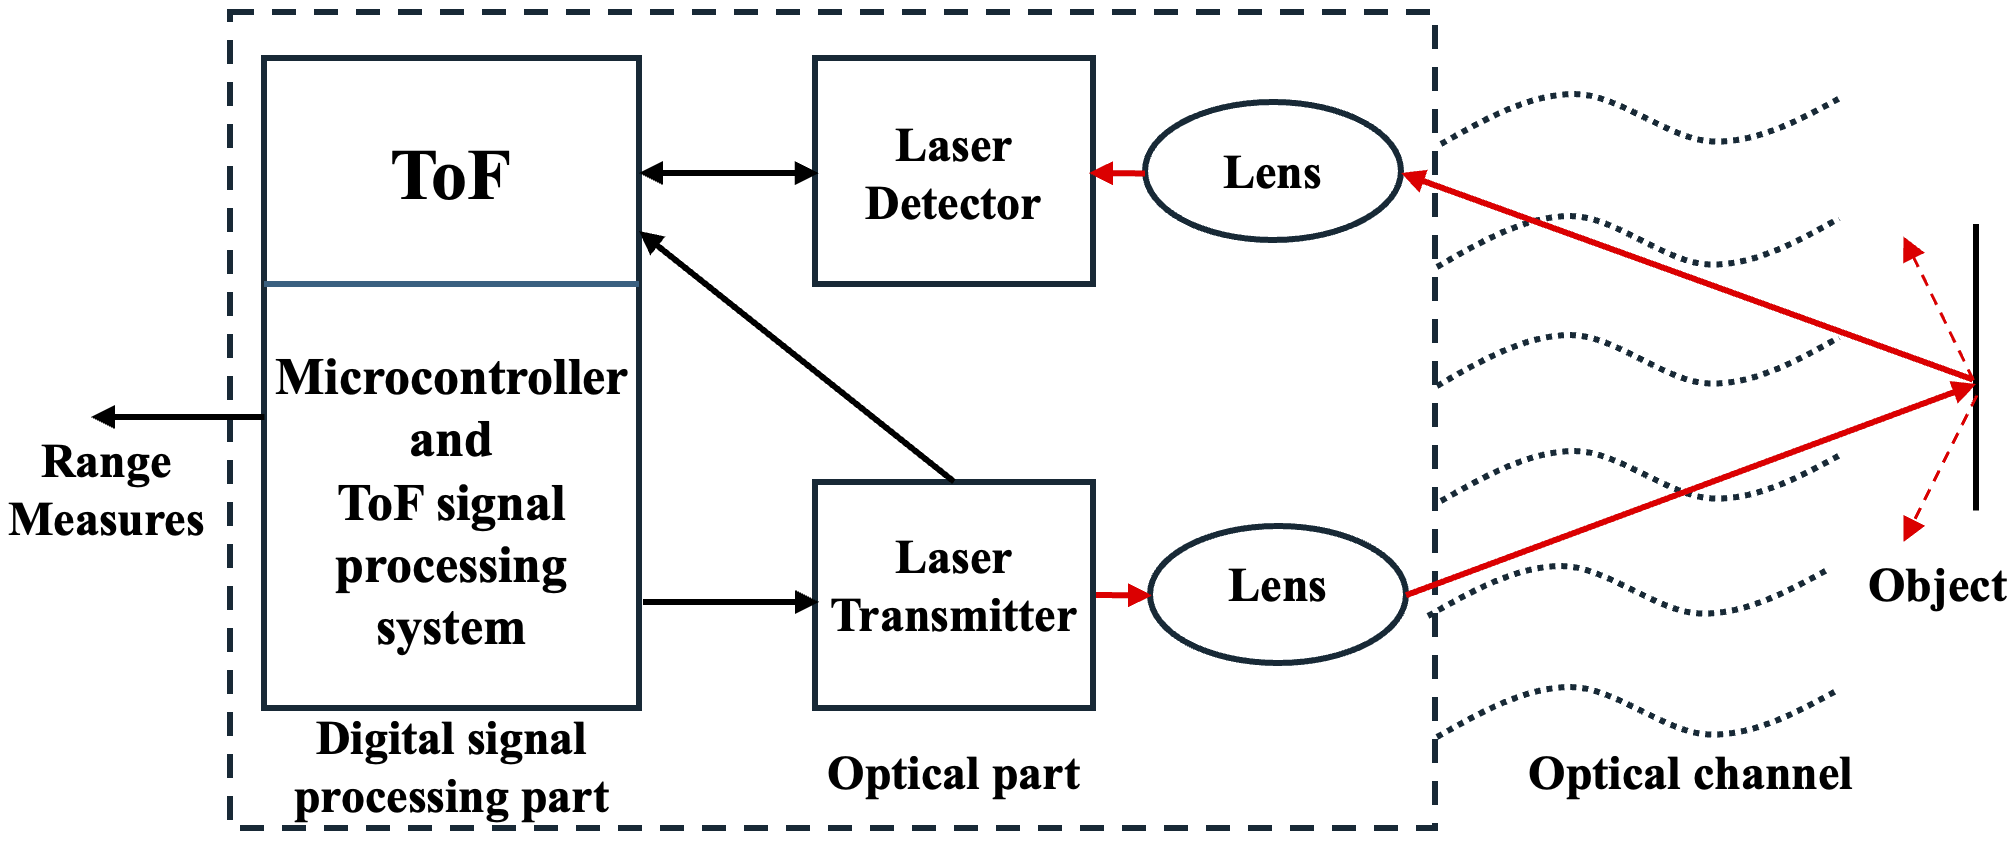
\includegraphics[width=1\linewidth]{figs/tof.png}
    \caption{ToF LiDAR example, adapted from~\cite{lidarexample}}
    \label{fig:lidar_example}
\end{figure}

\subsection{Depth Camera}
Common depth cameras, such as the Intel RealSense Camera, use these lenses to assess depth: 
a camera, an infrared (IR) camera, and an IR projector. 
They detect infrared light reflected from the object or body in front of them. 
The resulting visual data is combined with software to generate a depth estimate, 
which is then returned as a depth image~\cite{depthcam}.

\begin{figure}[H]
    \centering
    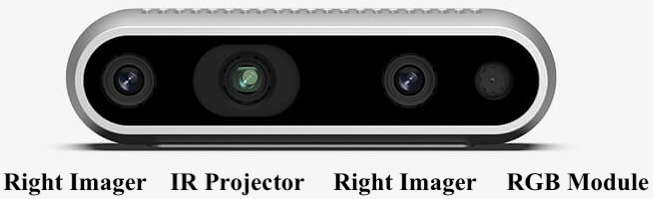
\includegraphics[width=1.0\linewidth]{figs/realsense.jpg}
    \caption{Intel RealSense camera}
\end{figure}

Different depth cameras achieve depth values through various techniques and mechanisms. 
Stereo vision systems use two spaced apart cameras to capture images from slightly different angles, 
similar to human binocular vision~\cite{kinect}. 
The system can calculate depth by comparing these two images and using the difference between corresponding points in the images. 
Structured light technology is the process of projecting a pattern of light (usually infrared) onto a scene and photographing it. 
The depth values are calculated by analysing the distortion of the light pattern caused by the surfaces in the scene~\cite{rgbdmapping}.
The ToF camera emits pulses of light (usually infrared) and measures the time it takes for the light to travel to the object and return to the camera~\cite{tof}. 
This is very similar to the principle of section~\ref{subsec:lidar} outlined above.

\subsection{SLAM}
\label{subsec:slam}
The availability of accurate maps enables system designs to operate in complex environments using only onboard sensors, 
rather than external reference systems (e.g., GPS). 
Over the last few decades, the robotics community has focused heavily on developing maps of indoor environments, often without the use of GPS~\cite{slam}. 
The simultaneous localization and map building (SLAM) problem is commonly used to describe the process of learning maps under attitude uncertainty~\cite{slamoverview}. 
It is a technique that allows robots to map unknown environments while also localising themselves based on the maps created, 
often in the absence of an external positioning system~\cite{slamii}.

SLAM combines data from various sensors 
(e.g., cameras, LiDAR, inertial measurement units) to create a consistent map of the environment and calculate the robot's position in relation to that map. 
The process consists of two major steps: localization (estimating the robot's position in the environment) and mapping (building a model or map of the environment's layout).

The SLAM algorithm is heavily reliant on odometry data, which measures changes in position over time. 
In this project, detailed odometry information is obtained by tracking the rotation of each wheel using a differential wheel. 
Differential steering provides the mobility and manoeuvrability required to navigate complex environments, 
and when combined with SLAM, it allows for precise navigation and obstacle avoidance in dynamic settings~\cite{slamtutorial}. 
Also, using only differential wheels as SLAM odometers amplifies the importance of obstacle avoidance for robots, 
as they are very sensitive to collisions. This is mentioned in following section~\ref{sec:result_and_discussion}.

\subsection{ROS2 Humble}
ROS 2 Humble Hawksbill is a version of the Robotics Operating System (ROS 2).
It is the successor to the original ROS (Robotics Operating System) and is intended to improve on its predecessor's functionality,
focusing on new robotics use cases, more robust communications, and support real-time systems~\cite{ros2}.
ROS2 Humble is used throughout this project for the following reasons: ROS 2 Humble is an LTS release, 
which means it will be supported and updated for a longer period of time. 
And when this project started, this version was the latest LTS version. 
Whilst it may be easier to find solutions within the ROS community when the project encounters problems using an earlier version, 
using a newer platform means that the project is more in line with the ongoing developments in the field of robotics, 
and thus easier to integrate with future technologies and standards emerging in the community. This is also a mission of this project.

\subsection{Gazebo}
Gazebo is a popular open-source robotics simulator with a powerful physics engine, high-quality graphics, 
and a wide range of sensors and objects that can be customised to simulate real-world scenarios. 
Furthermore, Gazebo includes a large library of sensor models and plug-ins for simulating cameras, LiDAR, 
and other common robotic sensors. The simulator is completely integrated with the Robotics Operating System (ROS), 
making it an excellent tool for developing and testing ROS-based applications in a simulated environment~\cite{gazebo}. 

This project uses the Gazebo simulation world throughout to run, test and correct the algorithms. 
This reduces the risks and costs associated with physical prototyping. 
And algorithms and robot interactions can be tested in a variety of scenarios without causing expensive hardware damage. 
Through simulation, it is possible to quickly iterate on algorithm design, test changes, and see the results immediately. 
This rapid feedback loop significantly accelerates the development process.
\begin{figure}[H]
    \centering
    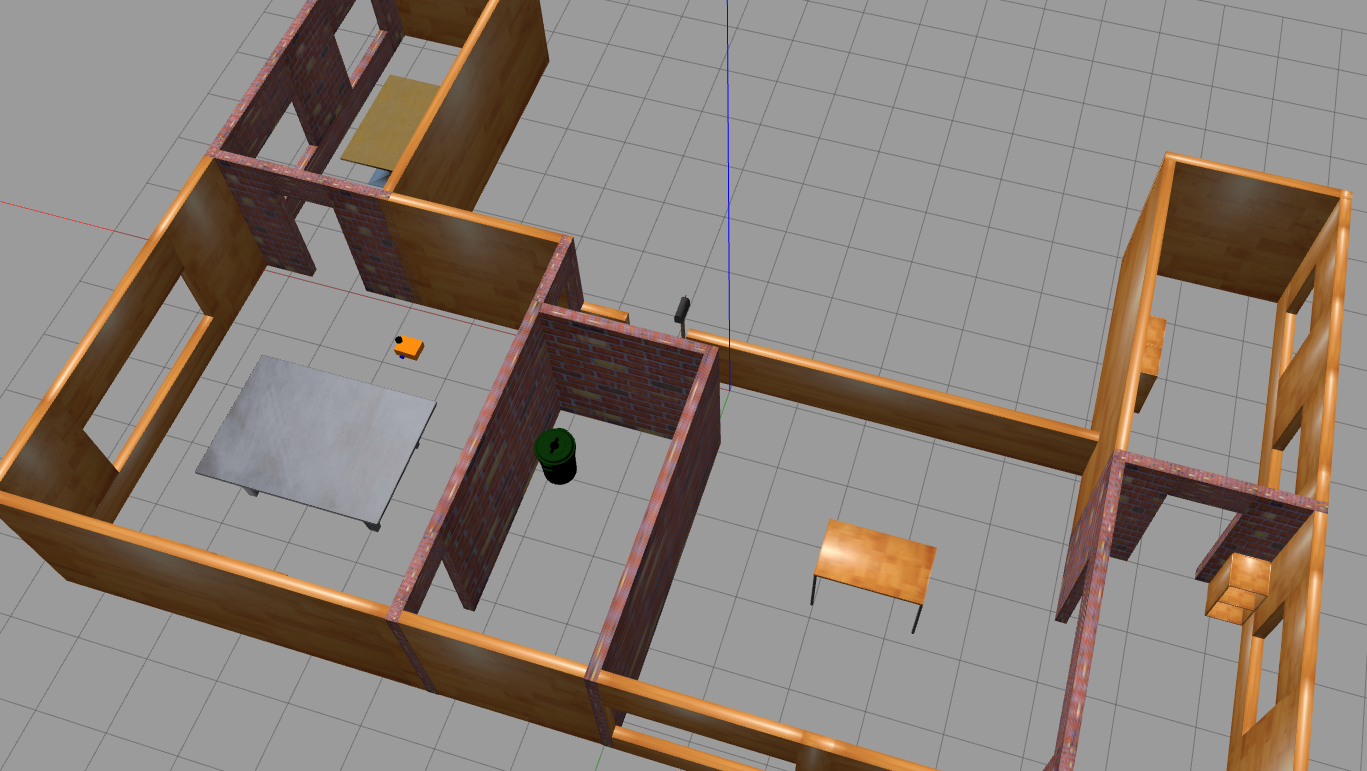
\includegraphics[width=0.76\linewidth]{figs/gazebo_house.png}
    \caption{Simulated indoor environment in Gazebo}
\end{figure}
\subsection{RViz2}
RViz is a powerful 3D visualisation tool for representing sensor data, robot state, and behaviour.
RViz2's displays can be customised to meet specific requirements, 
allowing it to adapt to a wide range of robotic applications~\cite{rviz2}. 
It is also fully integrated with ROS2 and it is compatible with Gazebo. 

RViz2 is used throughout this project to visualise data including robot models, 
trajectories, and sensor data streams (e.g. laser scans and cameras). 
It provides visual insights into what the robot is ``seeing'' and ``thinking'', 
which is essential for tuning algorithms and ensuring that they perform as expected.
\begin{figure}[H]
    \centering
    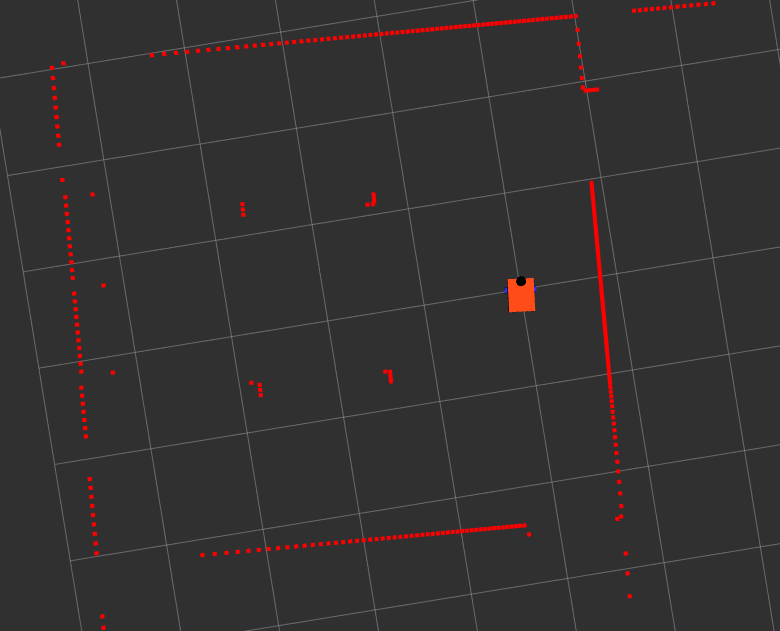
\includegraphics[width=0.8\linewidth]{figs/robotandlaser.png}
    \caption{The robot model and laserScan data visualised in RViz2}
\end{figure}
\subsection{Depthimage\_to\_Laserscan}
Depthimage\_to\_Laserscan is a ROS package that provides a simple solution for converting depth images from depth cameras to 2D laser scan data~\cite{rosdepthimage}. 

The principal of algorithm for converting depth image data to LaserScan data in the following section is adapted from this package. 
The details are explained in more detail below.

\subsection{Navigation2}
Because the primary goal of this project is to address the shortcomings of 2D LiDAR, 
it is important to employ an auto-navigation method that is well-suited to a wide range of sensors, 
simple to use, and provides reliable performance.
The Navigation2 framework is a cutting-edge, 
open-source navigation stack that includes a comprehensive set of tools and libraries 
for enabling autonomous navigation on a variety of robotic platforms, particularly in complex and dynamic environments~\cite{nav2}. 

Nav2 is user-friendly, with plug-and-play components 
that make it easier to set up and configure advanced navigation systems in robots. 
It offers a variety of navigational functions, 
such as path planning, obstacle avoidance, and map management. Its modular design makes it extremely scalable~\cite{nav2doc}. 
In this project, the navigation function of Navigation2 is used for simple robot navigation. 
The robot is only given a target position and then can plan an obstacle avoidance route through the given map.
\subsection{Slam\_toolbox}
As mentioned in section~\ref{subsec:slam}, SLAM is a central part of robot navigation. SLAM\_toolbox is a package for ROS. 
It provides tools to perform SLAM using various sensor data sources, both on real robots and in the simulated world~\cite{slamtoolbox}.

This package is used throughout the project in conjunction with the other tools mentioned above to implement robot navigation and map building.

\subsection{Proposed Solutions}
In the early stages of the project, two unique proposed solutions were also proposed and they are:
\subsubsection{YOLO-V8}
YOLO (You Only Look Once) is a deep learning model. 
It can detect objects, especially a wide variety of obstacles, with high accuracy and speed. 
Its superior efficiency enables robots to make fast, informed decisions about obstacle avoidance and path planning~\cite{yolo}.

However, whilst YOLOv8 provides powerful target detection capabilities, 
it relies heavily on visual data from the camera. 
The aim of this project was to explore sensor fusion. In particular, the integration of camera and LiDAR data, 
to take advantage of the complementary strengths of the two sensing modalities. 
YOLOv8 focuses only on camera input, which is not in line with the sensor fusion goals of this project.
\subsubsection{ORB-SLAM3}
ORB-SLAM (Oriented FAST and Rotated BRIEF SLAM) is a versatile and accurate visual SLAM method 
that utilises a feature-based approach for simultaneous localisation and mapping. 
It can construct detailed environmental maps and accurately locate vehicles in environments not recognised by GPS.

While ORB-SLAM is somewhat able to address the problem of map-building crashes due to collisions for robots using only differential wheel odometers
(the reason is explained in following section~\ref{sec:result_and_discussion}),
it is not primarily designed for dynamic obstacle detection and avoidance. 
Its main goal is to create the map of the environment, rather than consistently recognising and bypassing transient obstacles.
This is at odds with the goals of the project.
